\chapter{Comparing Conditional and Unconditional Diffusion Models}

\begin{figure}[b]
    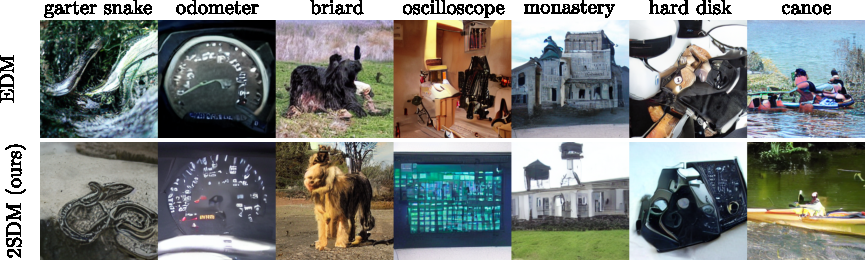
\includegraphics[width=\textwidth]{figs/2sdm/2SDM-main-fig.pdf}
    \caption{Class-conditional ImageNet-256 samples from our method, 2SDM, and a diffusion model baseline, EDM~\citep{karras2022elucidating}, both trained for 12 GPU days. Samples within the same column are generated with the same random seed and class label. In most columns the samples from 2SDM are visibly better, agreeing with the FIDs reported in \cref{sec:2sdm-experiments}.}
    \label{fig:latent-imagenet-samples}
\end{figure}


\begin{figure}[t]
    \centering
    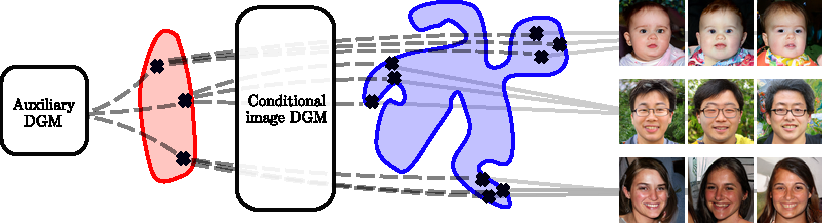
\includegraphics{figs/2sdm/vcdm-diagram.pdf}
    \caption{Visualization of 2SDM's generation process. First the auxiliary DGM samples a CLIP embedding, corresponding to a cross in the space of CLIP embeddings (red) in our illustration. Next, our conditional image model maps from the sampled CLIP embedding to a sampled image, visualized on the image manifold (blue). The distribution over plausible images is complex and multi-modal but becomes simpler when conditioned on a CLIP embedding. On the right we show three rows of sampled images. Within each row, all images are generated given the same CLIP embedding.}
    \label{fig:samples}
\end{figure}


\label{sec:2sdm-intro}
Recent text-to-image diffusion generative models (DGMs) have exhibited stunning sample quality~\citep{saharia2022photorealistic} to the point that they are now being used to create art~\citep{oppenlaender2022creativity}. 
%
Further work has explored conditioning on scene layouts~\citep{zhang2023adding}, segmentation masks~\citep{zhang2023adding,hu2022self}, or the appearance of a particular object \citep{ma2023unified}. We broadly lump these methods together as ``conditional'' DGMs to contrast them with ``unconditional'' image DGMs which sample an image without dependence on text or any other information.
%
Relative to unconditional DGMs, conditional DGMs typically produce more realistic samples~\citep{ho2022classifier,bao2022conditional,hu2022self} and work better with few sampling steps~\citep{meng2022distillation}. Furthermore our results suggest that sample realism grows with ``how much'' information the DGM is conditioned on. We therefore distinguish between ``strongly-conditional'' generation, where we condition on a high-dimensional feature like a long text prompt, and ``lightly-conditional'' generation, where
\begin{wrapfigure}[16]{r}{0.5\textwidth}
    \centering
    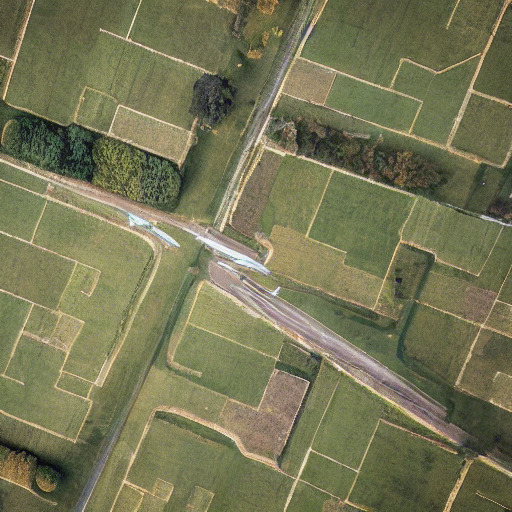
\includegraphics[width=0.24\textwidth]{figs/2sdm/uncond-aerial-photo.jpg}
    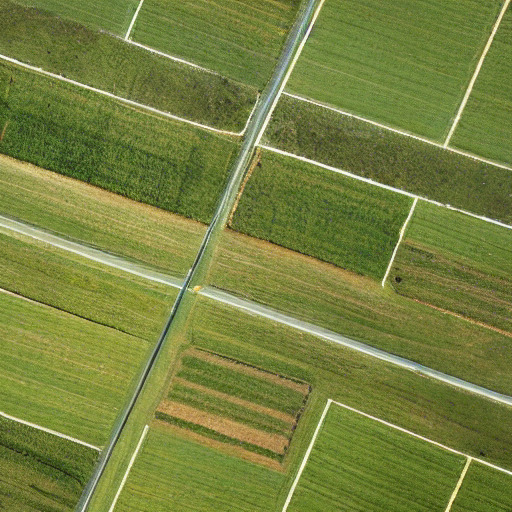
\includegraphics[width=0.24\textwidth]{figs/2sdm/cond-aerial-photo.jpg}
    \caption{\textbf{Left:} Output from Stable Diffusion~\citep{rombach2022high} prompted to produce ``aerial photography''. \textbf{Right:} Using a more detailed prompt\protect\footnotemark with the same random seed removes the ``smudged'' road artifact that appears on the left. 2SDM builds on this observation.}
    \label{fig:stable-diffusion-example}
\end{wrapfigure}
we condition on a lower dimensional feature like a class label or short text prompt. As hinted at in \cref{fig:stable-diffusion-example} an image is likely to be more realistic if conditioned on being ``an aerial photograph of a road between green fields'' (strongly-conditional generation) than if it is if simply conditioned on being ``an aerial photograph'' (lightly-conditional generation). 

% We therefore further distinguish between ``strongly-conditional'' image generation, where the image is conditioned on e.g. a long text prompt, which works well, and ``lightly-conditional'' generation, where the image is conditioned on a lower-dimensional feature like a class label or short text prompt, which works less well.



\footnotetext{We used the prompt ``Aerial photography of a patchwork of small green fields separated by brown dirt tracks between them. A large tarmac road passes through the scene from left to right.''}
This gap in performance is problematic. Imagine you need to sample a dataset of synthetic aerial photos.\footnote{ This may be done to, e.g., later train state-of-the-art a classification system~\citep{azizi2023synthetic}.}. A researcher doing so would currently have to either (a) make up a scene description before generating each dataset image, and ensure these cover the entirety of the desired distribution, or (b) accept the inferior image quality gleaned by conditioning just on each image being ``an aerial photograph''.  \Cref{fig:stable-diffusion-example} shows that the difference in quality can be stark.

We argue that a solution to this problem comes from revisiting the methodology of DALL-E 2, also known as unCLIP~\citep{ramesh2022hierarchical}. UnCLIP is a method for text-conditional image generation which we describe in detail in \cref{sec:2sdm-background}. It was originally proposed as a way to ``invert'' a pretrained CLIP embedder and thereby map from text to image space but, perhaps due to improved text embeddings and a desire for methodological simplicity, we are not aware of future work building on the two-stage unCLIP approach~\citep{rombach2022high,chang2023muse,hoogeboom2023simple}. We hope to counter this trend, arguing that, while unCLIP may provide little benefit for ``strongly-conditional'' text-to-image generation (especially when the text prompt is long or heavily ``prompt-engineered''), its benefits are in fact much greater than previously acknowledged when applied to unconditional or ``lightly-conditional'' generation.

Our final approach, based on unCLIP, is depicted in \cref{fig:samples}. A first ``auxiliary DGM'' samples vectors within an embedding space, with any vector describing a particular set of semantic characteristics of an image. The second stage, a ``conditional image DGM'', takes such a vector as input and samples an image with these semantic characteristics. The vector embedding is informative, as evidenced by the fact that all images within each row on the right of \cref{fig:samples}, which are all conditioned on the same embedding, look very similar. The conditional image DGM therefore inherits all the previously-described advantages of strongly-conditional DGMs even though our overall generative model is unconditional (or, with the generalization in \cref{sec:2sdm-method}, lightly-conditional). We call the resulting model a Two-Stage Diffusion Model (2SDM). 

\paragraph{Contributions} In \cref{sec:2sdm-background,sec:2sdm-cond-vs-uncond-dgms} we revisit unCLIP and then provide a novel explanation for why it is well-suited to the unconditional and lightly-conditional setting which was not explored by \citet{ramesh2022hierarchical}. We then demonstrate empirically that our lightly-conditional variant, 2SDM, yields large improvements on a variety of image datasets, tasks, and metrics in \cref{sec:2sdm-experiments}.

\section{Background} \label{sec:2sdm-background}
\paragraph{Conditional DGMs}
We provide a high-level overview of conditional DGMs that is sufficient to understand our contributions, referring to \citeauthor{karras2022elucidating} for a more complete description and derivation. A conditional image DGM~\citep{tashiro2021csdi} samples an image $\rvx$ given a conditioning input $\rvy$, where $\rvy$ can be, for example, a class label, a text description, or both of these in a tuple. We can recover an unconditional DGM by setting $\rvy$ to a null variable in the below. Given a dataset of $(\rvx,\rvy)$ pairs sampled from $\pdata(\cdot,\cdot)$, a conditional DGM $p_\theta(\rvx|\rvy)$ is fit to approximate $\pdata(\rvx|\rvy)$. It is parameterized by a neural network $\hat{\rvx}_\theta(\cdot)$ trained to optimize
\begin{align}\label{eq:diffusion-loss}
    % \mathcal{L}(\theta) = 
    \mathbb{E}_{u(\sigma)p_\sigma(\rvx_\sigma|\rvx,\sigma)\pdata(\rvx,\rvy)} \left[ \lambda(\sigma) \lvert\lvert \rvx - \hat{\rvx}_\theta(\rvx_\sigma, \rvy, \sigma) \rvert\rvert^2 \right]
\end{align}
where $\rvx_\sigma \sim p_\sigma(\cdot|\rvx,\sigma)$ is a copy of $\rvx$ corrupted by Gaussian noise with standard deviation $\sigma$; $u(\sigma)$ is a broad distribution over noise standard deviations; and $\lambda(\sigma)$ is a weighting function.
%
If $\lambda$ and $u$ are chosen appropriately, \cref{eq:diffusion-loss} is a lower bound on the data likelihood. It is common to instead set $\lambda$ and $u$ to values that maximize perceptual quality of the generated images but there remains  a close relationship to the ELBO~\citep{kingma2023understanding}. During inference, samples from $p_\theta(\rvx|\rvy)$ are drawn via a stochastic differential equation with dynamics dependent on $\hat{\rvx}_\theta(\cdot)$.



\paragraph{CLIP embeddings}
CLIP (contrastive language-image pre-training)~\citep{radford2021learning} consists of two neural networks, an image embedder $e_i(\cdot)$ and a text embedder $e_t(\cdot)$, trained on a large captioned-image dataset. Given an image $\rvx$ and a caption $\rvy$, the training objective encourages the cosine similarity between $e_i(\rvx)$ and $e_t(\rvy)$ to be large if $\rvx$ and $\rvy$ are a matching image-caption pair and small if not.
% The embedders are trained by separately embedding images and captions, and encouraging the cosine similarity between embeddings to be large if they are of matching image-caption pairs and small if not.
The image embedder therefore learns to map from an image to a semantically-meaningful embedding capturing any features that may be included in a caption. We use a CLIP image embedder with the ViT-B/32 architecture and weights released by \citet{radford2021learning}. We can visualize the information captured by the CLIP embedding by showing the distribution of images produced by our conditional DGM given a single CLIP embedding; see \cref{fig:samples}.

\paragraph{UnCLIP for text-to-image}
UnCLIP~\citep{ramesh2022hierarchical} uses the following text-to-image procedure: given a text prompt, it is embedded by a CLIP text embedder. A diffusion model then samples a plausible CLIP image embedding with high cosine similarity to this text image embedding. Finally, a conditional image diffusion model samples an image conditioned on CLIP image embedding and text prompt. This is described as ``inverting'' the CLIP embedder framework to map from image to text, hence the name unCLIP. In the next section we investigate when and why the quality of images produced by a CLIP-conditional image DGM may be greater than those generated by an unconditional image DGM.

\section{Conditional vs. unconditional DGMs} \label{sec:2sdm-cond-vs-uncond-dgms}
\paragraph{What does it mean to say that conditional DGMs beat unconditional DGMs?} A standard procedure to evaluate unconditional DGMs is to start by sampling a set of $N$ images independently from the model: ${\rvx^{(1)},\ldots,\rvx^{(N)} \sim p_\theta(\cdot)}$. We can then compute the Fr\'echet Inception distance (FID)~\citep{heusel2017gans} between this set and the dataset. If the generative model matches the data distribution well, the FID will be low.
%
For conditional DGMs the standard procedure has one extra step: we first independently sample ${\rvy^{(1)},\ldots,\rvy^{(N)} \sim \pdata(\cdot)}$. We then sample each image given the corresponding $\rvy^{(i)}$ as ${\rvx^{(i)} \sim p_\theta(\cdot|\rvy^{(i)})}$. 
%
Then, as in the unconditional case, we compute the FID between the set of images $\rvx_1,\ldots,\rvx_N$ and the dataset, without reference to $\rvy_1,\ldots,\rvy_N$. Even though it does not measure alignment between $\rvx, \rvy$ pairs, conditional DGMs beat comparable unconditional DGMs on this metric in many settings: class-conditional CIFAR-10 generation~\citep{karras2022elucidating}, segmentation-conditional generation~\citep{hu2022self}, or bounding box-conditional generation~\citep{hu2022self}.

\begin{figure}[t]
    \centering
    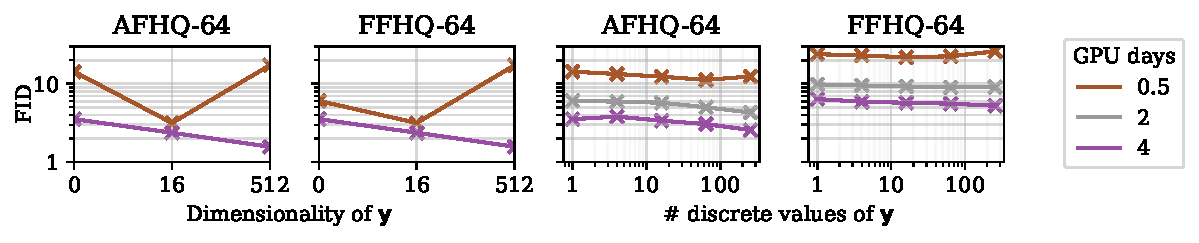
\includegraphics[width=\textwidth]{figs/2sdm/cond-results-vs-nclusters.pdf}
    \caption{FID versus dimensionality of $\rvy$ on AFHQ~\citep{choi2020stargan} and FFHQ~\citep{karras2018style}. With small training budgets (brown line), it is harmful when $\rvy$ is too informative. With larger training budgets (purple line), it is helpful to make $\rvy$ much more high dimensional.}
    \label{fig:fid-vs-ncomp}
\end{figure}

\paragraph{Why do conditional DGMs beat unconditional DGMs?}

Conditional DGMS ``see'' more data during training than their unconditional counterparts because updates involve $\rvy$ as well as $\rvx$. \citet{bao2022conditional,hu2022self} prove that this is not the sole reason for their successes because the effect holds up even when $\rvy$ is derived from an unconditional dataset through self-supervised learning.
%
To our knowledge, the best explanation for their success is, as stated by \citet{bao2022conditional}, that conditional distributions typically have ``fewer modes and [are] easier to fit than the original data distribution.''

\paragraph{When do conditional DGMs beat unconditional DGMS?}
%
We present results in \cref{fig:fid-vs-ncomp} to answer this question. We show FID scores for conditional DGMs trained to condition on embeddings of varying information content. 
%
We produce $\rvy$ by starting from the CLIP embedding of each image in our dataset and using either principal component analysis to reduce their dimensionality (left two panels) or K-means clustering to discretize them (right two panels)~\citep{hu2022self}.
%
We see that, given a small training budget, it is best to condition on little information. With a larger training budget, performance appears to improve steadily as the dimensionality of $\mathbf{y}$ is expanded. We hypothesize that \textbf{(1)} conditioning on higher-dimensional $\mathbf{y}$ slows down training because it means that points close to any given value of $\mathbf{y}$ will be seen less frequently and $\textbf{(2)}$ with a large enough compute budget, any $\mathbf{y}$ correlated with $\mathbf{x}$ will be useful to condition on. This suggests that, as compute budgets grow, making unconditional DGM performance match conditional DGM performance will be increasingly useful.

\paragraph{A perspective on unCLIP}
Recall that unCLIP leverages a CLIP-conditional generative model even when the original task calls for only a text-conditional image generative model. In light of this section, it makes sense that this should provide a benefit as long as the combination of text and CLIP embedding contains ``more'' information than the text prompt alone, which will always be the case. However, the disparity is even larger if we compare the CLIP-conditional generative model with an unconditional generative model  (i.e. one conditioned on zero bits of information). The unCLIP approach can therefore be expected to provide larger benefits for unconditional (or lightly-conditional) generation than for the text-conditional setting in which it was developed.


\section{Method} \label{sec:2sdm-2sdm-method}
% We have established that conditioning on CLIP embeddings improves DGMs. We now point out that this fact can be seen as a significant reason for unCLIP's success; it
We now formally introduce 2SDM, a variant of unCLIP for the unconditional setting. Recall that, for unconditional generation, the user does not wish to specify any input to condition on and, for the lightly-conditional setting, any such input is low-dimensional. We will denote any input $\rva$ (letting $\rva$ be a null variable in the unconditional setting) and from now on always use $\rvy := e_i(\rvx)$ to refer to a CLIP embedding. To make this deterministic encoding compatible with a probabilistic generative modeling perspective, we consider a joint distribution $\pdata(\rvx, \rvy, \rva)=\pdata(\rvx, \rva)\delta_{e_i(\rvx)}(\rvy)$, where $\pdata(\rvx, \rva)$ is described by a dataset and $\delta_{e_i(\rvx)}(\rvy)$ is a Dirac conditional distribution enforcing that $\rvy$ is the CLIP embedding of $\rvx$. From now on all distributions denoted with $\pdata$ should be understood as marginals and/or conditionals of this joint distribution, including our target distribution $\pdata(\rvx|\rva)$. 2SDM approximates this target distribution as
%
\begin{align} \label{eq:no-a}
    \pdata(\rvx|\rva) &= \mathbb{E}_{\pdata(\rvy|\rva)} \left[ \pdata(\rvx|\rvy,\rva) \right] \\
    &\approx \mathbb{E}_{p_\phi(\rvy|\rva)} \left[ p_\theta(\rvx|\rvy,\rva) \right] % = p_{\theta,\phi}(\rvx|\rva)
\end{align}
where $p_\phi(\rvy|\rva)$ is a second DGM modeling the CLIP embeddings. We can sample from this distribution by sampling $\rvy\sim p_\phi(\cdot|\rva)$ and then leveraging the conditional image DGM to sample $\rvx \sim p_\theta(\cdot|\rvy,\rva)$ We then return $\rvx$ and make no further use of $\rvy$.
%
From now on we will call $p_\theta(\rvx|\rvy,\rva)$ the \textit{conditional image model} and $p_\phi(\rvy|\rva)$ the \textit{auxiliary model}. In our experiments the auxiliary model uses a small architecture relative to the conditional image model and so adds little extra cost.\footnote{For our ImageNet experiments, sampling from our auxiliary model takes 35ms per batch item. Sampling from our image model takes 862ms and so 2SDM has inference time only $4\%$ greater than our baselines.}



\begin{figure*}[t]
    \centering
    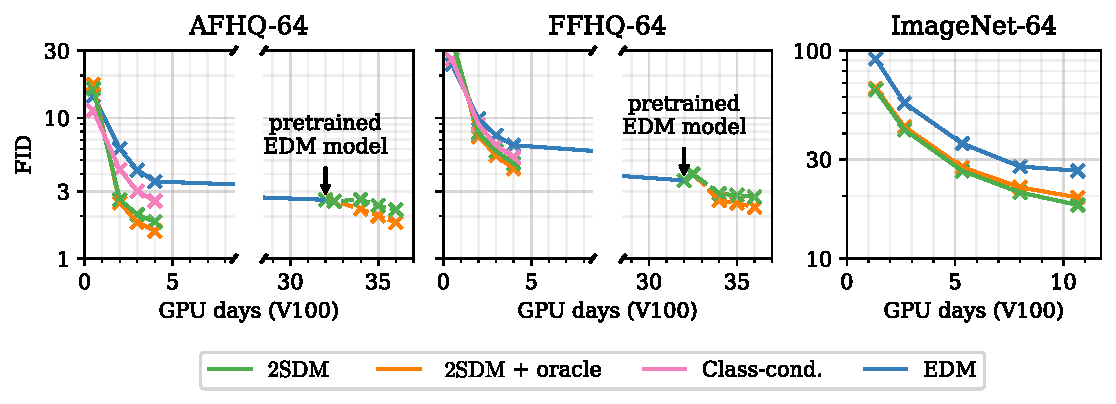
\includegraphics[width=\textwidth]{figs/2sdm/cond-results-1.pdf}
    \caption{FID throughout training. We show results for each method trained from scratch and, on AFHQ and FFHQ, for finetuning a pretrained EDM model (which was trained for the equivalent of 32 GPU days). 2SDM quickly outperforms EDM when trained from scratch and quickly improves on the pretrained model when used for finetuning.}
    \label{fig:fid_vs_training}
\end{figure*}

\paragraph{Auxiliary model}
Our auxiliary model is a conditional DGM targeting $\pdata(\rvy|\rva)$, where $\rvy$ is a 512-dimensional CLIP embedding. Following \cref{eq:diffusion-loss}, we train it by minimizing
\begin{equation}
\label{eq:auxiliary-model-objective}
    \mathbb{E}_{u(\sigma)p_\sigma(\rvy_\sigma|\rvy,\sigma)\pdata(\rvy,\rva)} \left[ \lambda(\sigma) \lvert\lvert \rvy - \hat{\rvy}_\theta(\rvy_\sigma, \rva, \sigma) \rvert\rvert^2 \right].
\end{equation}
Analogously to \cref{eq:diffusion-loss}, $\rvy_\sigma \sim p_\sigma(\cdot|\rvy,\sigma)$ is a copy of the CLIP embedding $\rvy$ corrupted with Gaussian noise, and $u$ and $\rvy$ are the training distribution over noise standard deviations and weighting function respectively.
We follow the architectural choice of \citet{ramesh2022hierarchical} and use a DGM with a transformer architecture. It takes as input a series of 512-dimensional input tokens: an embedding of $\sigma$; an embedding of $\rva$ if this is not null; an embedding of $\rvy_\sigma$; and a learned query. These are passed through six transformer layers and then the output corresponding to the learned query token is used as the output. Like \citet{ramesh2022hierarchical}, we parameterize the DGM to output an estimate of the denoised $\rva$ instead of estimating the added noise as is more common in the diffusion literature.
%
On AFHQ and FFHQ we find that data augmentation is helpful to prevent the auxiliary model overfitting. We perform augmentations (including rotation, flipping and color jitter) in image space and feed the augmented image through $e_i(\cdot)$ to obtain an augmented CLIP embedding. Following \citet{karras2022elucidating}, we pass a label describing the augmentation into the transformer as an additional input token so that we can condition on there being no augmentation at test-time.

\paragraph{Conditional image model}
Including the additional conditioning input $\rva$, the conditional image model's training objective is
\begin{equation}
\label{eq:conditional-image-model-objective}
    \mathbb{E}_{u(\sigma)p_\sigma(\rvx_\sigma|\rvx,\sigma)\pdata(\rvx,\rvy,\rva)} \left[ \lambda(\sigma) \lvert\lvert \rvx - \hat{\rvx}_\theta(\rvx_\sigma, \rvy \oplus \rva, \sigma) \rvert\rvert^2 \right].
\end{equation}
where $\rvy \oplus \rva$ is the concatenation of $\rvy$ and $\rva$ to form a single vector which the image model is conditioned on. We match our diffusion process hyperparameters, including $u$ and $\lambda$, to those of \citet{karras2022elucidating}, and also use their proposed Heun sampler.  For AFHQ and FFHQ, we use the U-Net architecture originally proposed by \citet{song2020score}. For ImageNet, we use the slightly larger U-Net architecture proposed by \citet{dhariwal2021diffusion}. We match the data augmentation scheme to be the same as that of \citet{karras2022elucidating} on each dataset. There are established conditional variants of both architectures~\citep{dhariwal2021diffusion,karras2022elucidating} that add a learned linear projection to the embedding of the noise standard deviation $\sigma$.  We use the same technique to incorporate the concatenated conditioning inputs $\rvy\oplus\rva$.
% Our conditional image model needs to additionally incorporate $\rva$; we can do so by simply concatenating it to $\rvy$ and learning a projection for the resulting vector.



\section{Experiments} \label{sec:2sdm-experiments}


\begin{table}[t]
\centering
\caption{Comparison of 2SDM and EDM on a suite of metrics. Best performance for each metric and dataset is shown in bold. Higher is better for metrics marked $\uparrow$; lower is better for $\downarrow$. Results reported for EDM on FFHQ and AFHQ are computed with the pretrained checkpoints released by \citet{karras2022elucidating}. Results reported for 2SDM on FFHQ are with finetuning from this pretrained checkpoint. All others are trained from scratch.}
\begin{tabular}{lcccccccccc}
\toprule
 \multirow{2}{*}{Dataset} & \multirow{2}{*}{Method} & \multirow{2}{*}{\shortstack{Inception\\Score $\uparrow$}} & \multirow{2}{*}{Precision $\uparrow$} & \multirow{2}{*}{Recall $\uparrow$} & \multirow{2}{*}{FID $\downarrow$} & \multirow{2}{*}{sFID $\downarrow$} \\
 & & & & & & \\
\midrule
\multirow{2}{*}{AFHQ-64} & 2SDM & $\mathbf{10.00}$ & $\mathbf{0.844}$ & $\mathbf{0.619}$ & $\mathbf{1.56}$ & $13.7$ \\
 & EDM & $8.91$ & $0.752$ & $0.614$ & $2.04$ & $13.7$ \\
\midrule
\multirow{2}{*}{FFHQ-64} & 2SDM & $\mathbf{3.47}$ & $\mathbf{0.721}$ & $\mathbf{0.697}$ & $\mathbf{2.32}$ & $4.98$ & \\
 & EDM & $3.33$ & $0.697$ & $0.569$ & $2.46$ & $\mathbf{4.90}$ \\
\midrule
\multirow{2}{*}{\shortstack[l]{Class-cond. \\ ImageNet-64}} & 2SDM & $\mathbf{17.3}$ & $\mathbf{0.541}$ & $\mathbf{0.573}$ & $\mathbf{17.4}$ & $\mathbf{4.63}$ \\
 & EDM & $13.6$ & $0.530$ & $0.532$ & $25.4$ & $6.50$ \\
\midrule
\multirow{2}{*}{\shortstack[l]{Uncond. \\ ImageNet-64}} & 2SDM & $\mathbf{15.6}$ & $\mathbf{0.614}$ & $\mathbf{0.526}$ & $\mathbf{21.0}$ & $\mathbf{5.59}$ \\
 & EDM & $11.3$ & $0.523$ & $0.524$ & $35.1$ & $9.14$ \\
 \midrule
\multirow{2}{*}{\shortstack[l]{Class-cond. latent \\ ImageNet-256}} & 2SDM & $\mathbf{52.1}$ & $\mathbf{0.590}$ & $0.603$ & $\mathbf{24.3}$ & $\mathbf{7.36}$ \\
 & EDM & $40.4$ & $0.532$ & $\mathbf{0.610}$ & $34.2$ & $9.59$ \\
\end{tabular}
\label{tab:2sdm-many-metrics}
\end{table}

\paragraph{Experimental setup and results overview}
%\begin{table}
We perform experiments in five settings: unconditional AFHQ modeling at $64\times64$ resolution~\citep{choi2020stargan}; unconditional FFHQ modeling at $64\times64$ resolution~\citep{karras2018style}; unconditional ImageNet modeling at $64\times64$ resolution~\citep{deng2009imagenet}; class-conditional ImageNet modeling at $64\times64$ resolution; and finally class-conditional latent ImageNet modeling at $256\times256$ resolution, in which we train the diffusion models in the latent space of the pretrained VAE used by Stable Diffusion~\citep{rombach2022high}. In every setting, we compare against EDM~\citep{karras2022elucidating}, a standard DGM directly modeling $\pdata(\rvx|\rva)$, with an identical architecture to 2SDM. We match the training compute of our conditional image model with that of EDM in every case. The auxiliary model is trained for one day on a single V100 GPU so adds little additional cost. On AFHQ and FFHQ, we match the EDM parameters to those of \citet{karras2022elucidating}. On ImageNet-64, we have a smaller training budget and so decrease the batch size to 128 and the learning rate to $1\times10^{-4}$. For simplicity we match 2SDM to use the same learning rate and batch size.

For the first three of our listed settings, \cref{fig:fid_vs_training} reports the FID throughout the training of the conditional image diffusion model (or image DGM baseline).\footnote{Each FID in \cref{fig:fid_vs_training} is estimated using $20\,000$ images, each sampled with the SDE solver proposed by \citet{karras2022elucidating} using 40 steps, $S_\text{churn}=50$, $S_\text{noise}=1.007$, and other parameters set to their default values. Our other reported FID scores use $50\,000$ samples, as is standard, and the same sampler hyperparameters.}  In each case, the auxiliary model is trained for one day on one V100 GPU. We consider training the conditional image model from scratch (for up to 4 GPU days on AFHQ and FFHQ, or up to 11 GPU days on ImageNet-64), and see that it improves upon our EDM baseline for any training budgets over 1-2 GPU days. For AFHQ, this improvement is so substantial that 2SDM's FID after two GPU days is better than that of the pretrained EDM model released by \citet{karras2022elucidating}, which was trained for the equivalent of 32 V100 GPU days. In addition to training from scratch, on AFHQ and FFHQ we consider initializing 2SDM's training from the pretrained EDM checkpoints. To do so, we simply add a learnable linear projection of the CLIP embedding and initialize its weights to zero. We see that this allows for a fast and significant improvement in FID over the baseline in each case. We note, though, that training 2SDM from scratch for 4 GPU days 
\begin{wraptable}{r}{0.6\textwidth}
%\vspace{-.4cm}
\centering
\caption{A comparison of FID with the state-of-the-art (SOTA) in bold. EDM (single seed) is our re-computation of the EDM's reported results using a single seed instead of taking the best of three.}
\label{tab:2sdm-sota}
\begin{tabular}{lccc}
\midrule
Dataset         & AFHQ-64 & FFHQ-64 \\
\midrule
PFGM++~\citep{xu2023pfgm++}          & $-$ & $2.43$ \\
EDM~\citep{karras2022elucidating}
& $1.96$ & $2.39$  \\
EDM (single seed)     & $2.04$ & $2.46$  \\
EDM-G++~\citep{kim2022refining}               & $-$    & $\mathbf{1.77}$  \\
2SDM            & $\mathbf{1.56}$ & $2.31$ \\
% \hline
% \textit{Overfit 2SDM}    & $\mathit{1.16}$ & $\mathit{3.33}$ \\
\end{tabular}
%\end{table}
\end{wraptable}
outperforms 4 GPU days of finetuning on AFHQ and so recommend training 2SDM from scratch when sufficient compute is available.

\Cref{fig:fid-vs-ncomp} also compares against ``2SDM + oracle'', which is a supposed upper bound on 2SDM's performance given by sampling a CLIP image embedding from an oracle (in practice, the dataset) and then using 2SDM's conditional image model to sample an image conditioned on it. It therefore describes the performance that 2SDM would achieve with a perfect auxiliary model. On AFHQ-64, 2SDM with an oracle achieves a FID $56\%$ lower than EDM. Without an oracle, 2SDM still achieves a FID $48\%$ lower than 2SDM. We therefore say that 2SDM yields an improvement $87\%$ as large as can be gleaned by using a purely conditional DGM. Similarly for FFHQ, 2SDM obtains an improvement $81\%$ as large as is possible with a purely conditional DGM.\footnote{See \cref{tab:2sdm-results-breakdown} for the FIDs used in these calculations.} We can therefore say that our cheaply-trained auxiliary model is good enough to allow us to capture the majority of the benefits of conditional generation for the unconditional generation task. Intriguingly,
 on ImageNet-64, 2SDM achieves better FID \textit{without} an oracle. This suggests that imperfections in the distribution
learned by the auxiliary model improve the visual quality of the generated images. We observed this trend consistently on ImageNet, and believe that characterizing exactly when and why it occurs is an intriguing direction for future work.

Finally, \cref{fig:fid_vs_training} also compares against ``Class-cond'', which is an ablation of 2SDM in which we replace the CLIP embedding $\rvy$ with a single discrete label obtained by K-means clustering of the CLIP embedding (as on the right of \cref{fig:fid-vs-ncomp}). For unconditional generation tasks, we can then replace our auxiliary model with a simple categorical distribution modeling $\pdata(\rvy|\rva)=\pdata(\rvy)$ similarly to \citet{hu2022self}, simplifying the generative procedure. We see that this baseline is outperformed by 2SDM, justifying our choice to use a continuous $\mathbf{y}$.

We report our final FIDs on AFHQ and FFHQ alongside the state-of-the-art in \cref{tab:2sdm-sota}. Despite our limited training budget, our results on AFHQ beat the state-of-the-art and our results on FFHQ come second to EDM-G++~\citep{kim2022refining}, a potentially orthogonal approach to improving EDM.

\paragraph{Latent diffusion on ImageNet-256}
% 2SDM bears some similarities to a latent diffusion model~\citet{rombach2022high}: its auxiliary model learns a distribution over learned embeddings, similarly to the diffusion component of a latent diffusion model. 
We combine 2SDM and the latent diffusion modeling framework~\citep{rombach2022high} on the ImageNet-256 dataset as follows. We take the pretrained Stable Diffusion VAE encoder and decoder released by \citet{rombach2022high}. We feed a $256\times256\times3$ dataset image through the VAE encoder to create $64\times64\times4$ tensors, which we use as the training targets $\rvx$ for our conditional image model. The training targets for the CLIP embeddings $\rvy$ are created by embedding the $256\times256\times3$ images with the standard CLIP image embedder. We use the ImageNet class labels as additional inputs $\rva$. At test time, we take $\rva$ as an input; we then sample $\rvy$ given $\rva$ from our auxiliary model; we then sample $\rvx$ given $\rvy$ and $\rva$ from our conditional image model; we finally use the Stable Diffusion VAE decoder to produce an image given $\rvx$. Samples from this version of 2SDM, as well as our EDM baseline operating in the same latent space, are shown in \cref{fig:latent-imagenet-samples}. While the compute used for each (12 GPU days) is far from that of the state-of-the-art for this dataset, the samples from 2SDM are noticeably better, supporting the FID scores in \cref{tab:2sdm-many-metrics}.

\paragraph{Diverse metrics}
In \cref{tab:2sdm-many-metrics} we show a comparison of 2SDM and EDM on a variety of metrics. The Inception Score~\citep{salimans2016improved,barratt2018note} measures the diversity of the output from an image classifier when run on sampled images. The Precision and Recall metrics~\citep{kynkaanniemi2019improved} estimate, roughly speaking, the proportion of generated images that lie on the data manifold (Precision) and the proportion of dataset images that can be found within the manifold of generated images (Recall). The FID approximates the distance between the distribution of embeddings of dataset images and that of embeddings of generated images. The sFID is similar but uses an embedding with more spatial information. 2SDM outperforms EDM on 22 of the 25 metric-dataset combinations, and is outperformed on only 2.
%2SDM always performs better in terms of inception score, precision, and FID.

\paragraph{Comparison of relative improvements between tasks}
In terms of FID, and for the networks trained from scratch and matched for training compute, the percentage improvement of 2SDM over EDM is $48.2\%$ on AFHQ-64; $26.0\%$ on FFHQ-64; $31.5\%$ on class-conditional ImageNet-64; $40.2\%$ on unconditional ImageNet-64; and $28.9\%$ on class-conditional ImageNet-256. While these are all substantial improvements, we point out two comparisons in particular. 

First, the gain from using 2SDM on unconditional ImageNet-64 ($40.2\%$) is greater than that on class-conditional modeling of the same dataset ($31.5\%$). This supports our argument that two-stage diffusion techniques like 2SDM can have even greater impact in unconditional (or lightly-conditional) generation than in the text-conditional (or strongly-conditional) setting in which they were originally introduced with unCLIP~\citep{ramesh2022hierarchical}.  Noting that the class label already contains some of the information stored in a CLIP embedding, this finding also fits with our discussion of the effects of conditioning in \cref{sec:2sdm-2sdm-cond-vs-uncond-dgms}. The performance of an image model conditioned on just a class label (EDM on class-cond. ImageNet) should therefore be somewhere in between that of an unconditional image model (EDM on uncond. ImageNet) and that of a CLIP-conditional image model (2SDM, assuming the auxiliary model is good), leading to this finding.

Second, the $28.9\%$ improvement in performance for the latent diffusion model on ImageNet-256 is only slightly less than the $31.5\%$ improvement for pixel-space diffusion on class-conditional ImageNet-64. This confirms that 2SDM can be readily combined with the widely used latent diffusion framework.

\paragraph{Inference speed}
Sampling from 2SDM does impose a small additional cost relative to EDM, since we must begin by sampling from the auxiliary model. In all experiments, when we use 40 diffusion steps, sampling from our auxiliary model takes 8.8s with batch size 256. This corresponds to 35ms per batch item. Our conditional image model and our EDM baseline use identical architecture (other than the projection of $\rvy$) and we could not detect a difference between their sampling timeswhich were 862ms per batch item on our ImageNet architecture and 789ms per batch item on our AFHQ and FFHQ architecture. This means that the increase in time due to using 2SDM instead of EDM is less than $4\%$. Furthermore, we can negate this increase by using two less sampling steps for the conditional image model. \Cref{tab:2sdm-fid-and-time} in the appendix shows that this lets us make 2SDM faster than EDM with almost no effect on sample quality.

\paragraph{Overfitting analysis}
\begin{wrapfigure}[18]{r}{0.5\textwidth}
    \centering
    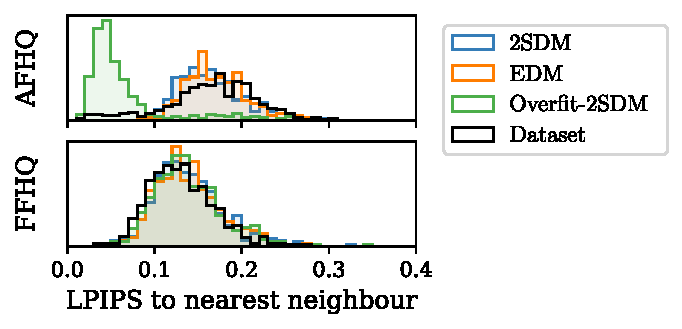
\includegraphics[width=0.5\textwidth]{figs/2sdm/afhq_ffhq.pdf}
    \caption{Distribution of LPIPS~\citep{zhang2018perceptual} distances to the nearest neighbour in the training set for sampled images from EDM, 2SDM, and Overfit-2SDM. We see clear signs of overfitting for Overfit-2SDM on AFHQ but not for any other methods or datasets. }
    \label{fig:overfit-2SDM-nearest-neighbours}
\end{wrapfigure}
We test for overfitting on AFHQ and FFHQ in the appendix through interpolation plots and nearest neighbour searches.
%Our results are summarized in \cref{fig:overfit-2SDM-nearest-neighbours}, which plots the distribution of distances to the training set nearest neighbour for images sampled by a variety of methods.
We summarize these results in \cref{fig:overfit-2SDM-nearest-neighbours} by sampling 100 images from each method; computing the LPIPS distance of each one to every training set image and taking the minimum over all training set images; and then plotting the histogram of these minima. To create the black line, we use 100 training set images and take the minima over \textit{non-zero} LPIPS distances to training set images to avoid them being reported as their own nearest neighbours. We can be confident that a method is overfitting if its curve is further to the left than the black curve. We see that both 2SDM and EDM ovefit slightly on AFHQ (which contains only $15\,000$ images) but no overfitting is visible on FFHQ (which has $70\,000$ images). Seeing as these plots are similar for 2SDM and EDM, and given that ImageNet is a much larger dataset than AFHQ and FFHQ, we are confident that 2SDM's gains do not come from overfitting. We do, however, include another method, Overfit-2SDM, as a point of interest and note of warning for future work on this topic. Overfit-2SDM is a variation of 2SDM in which we train the CLIP parameters jointly with the auxiliary and conditional image DGMs. It achieves state-of-the-art FID on AFHQ but, as we see in \cref{fig:overfit-2SDM-nearest-neighbours}, only through near-total overfitting to the training set. See the appendix for more details.



\section{Related work}
\textbf{Intermediate variables in diffusion models}~
 Our work takes inspiration from \citet{weilbach2022graphically}, % who use diffusion models to perform approximate inference in graphical models. They 
who show improved performance in various approximate inference settings by modeling problem-specific auxiliary variables (like $\rvy$) in addition to the variables of interest ($\rvx$) and observed variables ($\rva$). We apply these techniques to the image domain and incorporate pretrained CLIP embedders to obtain auxiliary variables. 

\textbf{Latent diffusion}~
2SDM also relates to methods which perform diffusion in a learned latent space~\citep{rombach2022high}: our auxiliary model $p_\phi(\rvy|\rva)$ is analogous to a ``prior'' in a latent space and our conditional image model $p_\theta(\rvx|\rva,\rvy)$ to a ``decoder'' Such methods typically use a near-deterministic decoder and so their latent variables must summarize all information about the image. Our conditional DGM decoder, on the other hand, is a DGM that will function reasonably however little information is stored in $\rvy$. This means that 2SDM provides an additional degree of freedom in terms of what to store. Furthermore, as we showed in \cref{sec:2sdm-experiments}, 2SDM can be fruitfully combined with latent diffusion.

\textbf{Self-supervised representations}~
\citet{bao2022conditional,hu2022self} both use self-supervised learning to obtain auxiliary variables and then training a diffusion model $p(\rvx|\rva)$. However, they do not model $\rva$ and therefore are not able to sample $\rvx$ without an oracle that can provide $\rva$. Their success when given an oracle, however, provides reason to believe that our approach is likely to yield benefits even if the embedder that produces $\rva$ is obtained through self-supervised learning and without access to additional (or multi-modal) data as our CLIP embedder was trained with.

\textbf{Integrating additional data}~
Our method can be understood as a means to leverage the ``world knowledge'' inside a CLIP embedder for improved performance on the image generation task. Another way in which additional knowledge, or data, could be leveraged is by training a multi-headed diffusion model which simultaneously approximates the score function and makes predictions of side information like class labels. \citet{deja2023learning} propose a method for doing so but do not demonstrate improved performance on the unconditional generation task.

\section{Discussion and conclusion}
We have demonstrated 2SDM, a variant of unCLIP for unconditional or lightly-conditional image generation, and argued that it has more benefits in this setting that in the text-conditional setting in which unCLIP was originally proposed. Therefore, even if the trend towards simple single-stage architectures continues for large-scale text-to-image models~\citep{rombach2022high,chang2023muse,hoogeboom2023simple}, unCLIP-style approaches could offer large jumps in performance for lightly-conditional image generation tasks.
%
2SDM also holds promise for improving video generation. This is a domain for which CLIP could be readily applied, and being able to learn relationships in the relatively low-dimensional CLIP embedding space could significantly increase training throughput relative to working purely in pixel (or VAE embedding) space.

A massive unexplored design space remains. For pedagogical purposes we intentionally kept 2SDM simple, using known diffusion architectures and objectives. It is likely that optimizing these design choices for the lightly-conditional 2SDM use-case would improve performance. In addition, there are almost certainly more useful quantities that we could condition on than CLIP embeddings. 
\citet{bao2022conditional,hu2022self} have shown that self-supervised learning techniques provide a promising avenue for obtaining useful ``latent'' representations. Exactly the properties that an embedding should have to be beneficial for techiques like 2SDM is another open question that is ripe for future work to tackle. Such a line of work may also fix one limitation of 2SDM, namely that it relies on the availability of a pretrained CLIP embedder. While this is freely available for natural images, it could be a barrier to other applications. Improvements may also be gleaned by conditioning on multiple quantities, or ``chaining'' a series of conditional DGMs together. An alternative direction is to simplify 2SDM's architecture by, for example, learning a single diffusion model over the joint space of $\rvx$ and $\rvy$ instead of generating them sequentially. 
%
We did not use classifier-free guidance~\citep{ho2022classifier} in this work, which can improve visual fidelity at the cost of losing the mass-covering behavior that diffusion models are known for. Conditioning on the CLIP embedding with a high guidance scale could help to optimize for visual quality in future work.
%


% \section{Ethics statement}
% Like much foundational research in modern generative modeling, this work carries risks like aiding the generation of deepfakes for dis- or misinformation campaigns. This leads to a second negative consequence: that trust in various forms of visual evidence, such as photographs, videos, and audio recordings, may no longer be possible. One avenue with which to address these consequences is research towards developing robust and effective methods for detecting and mitigating the harmful effects of deepfakes and synthetic media manipulation. Furthermore, increasing public awareness about the existence and potential impact of deepfakes can empower people to critically evaluate information and be more resilient to manipulation attempts. 2SDM has a potential risk on top of this: it leverages a publicly available "foundation model" in the form of a CLIP embedder to enhance the quality of generated content. Biases present in the foundation model may influence the outputs of 2SDM even if they are not present in the image dataset used for training. Stringent evaluation of foundation models may  mitigate potential harms arising from this.

% \section{Reproducibility statement}
% We release source code at \url{https://anonymous.4open.science/r/2sdm}. We will additionally release trained checkpoints on acceptance.